\section{Solução de Energia}
O grupo de engenharia de energia é responsável pela análise e escolha da fonte energética do projeto, pelo estudo do tempo de duração da carga desta fonte, bem como o dimensionamento do sistema fotovoltaico offgrid a ser instalado.


\subsection{Motor}
Neste projeto será utilizado o motor elétrico, que é uma máquina de construção simples,e que possui uma grande versatilidade de adaptação às cargas dos mais diversos tipos e potências.

Entre os tipos de motores estão os de corrente alternada e os de corrente contínua. Foi escolhido o de corrente contínua, pois apesar do seu custo mais elevado, ele funciona com velocidade ajustável entre amplos limites e se prestam a controles de grande flexibilidade e precisão.

\subsubsection{Dimensionamento do Motor}

Para a definição de capacidade de dosagem do sistema de dosagem, utilizou-se a equação abaixo \cite{agricola}:

\begin{equation}
Q=4,71.10^{-5}.(D^{2}-d^{2}).p.n
\end{equation}

Onde:


D = diâmetro da rosca tubular, cm;

Q = capacidade, $m³/h$;

d = diâmetro interno do helicóide, cm;

p = passo do helicóide, cm e

n = rotação, rpm.

\begin{equation}
Q=4,71.10^{-5}.(10^{2}-2,5^{2}).10.28
\end{equation}

Cálculo da potência requerida:

\begin{equation}
Pt = 2,22.10^{-4}.(Q.\mu.L.\emptyset)
\end{equation}

Onde:

Pt = potência requerida pelo transportador, cv;

Q = capacidade, $m^3/h$;

$\mu$ = massa específica do material, $kg/m^3$;

L = comprimento total do transportador, m e

$\emptyset$ = fator de potência adimensional.


\begin{equation}
Pt = 2,22*10^{-4}*(0,020605*243,66*1*0,4)
\end{equation}
\begin{equation}
Pt = 0,000447*2
\end{equation}
\begin{equation}
Pt = 0,0008941 \text{CV}
\end{equation}


A potência é multiplicada por 2, pois quando seu valor é menor que 1,0 , deve-se aplicar o fator de correção no valor de 2.

Cálculo do torque:

\begin{equation}
T=9550.\frac{Pt}{n}
\end{equation}

Onde:

T = torque, N.m;

Pt = potência requerida pelo transportador, kW;

Logo, o tem-se um torque requerido de $T=0,2017N.m$

\subsubsection{Motor DC}

O motor escolhido foi o da marca Bosh, modelo F006 B20 321, e foi acoplado à rosca helicoidal, como mostra a figura abaixo.

\begin{figure}[!h]
\centering 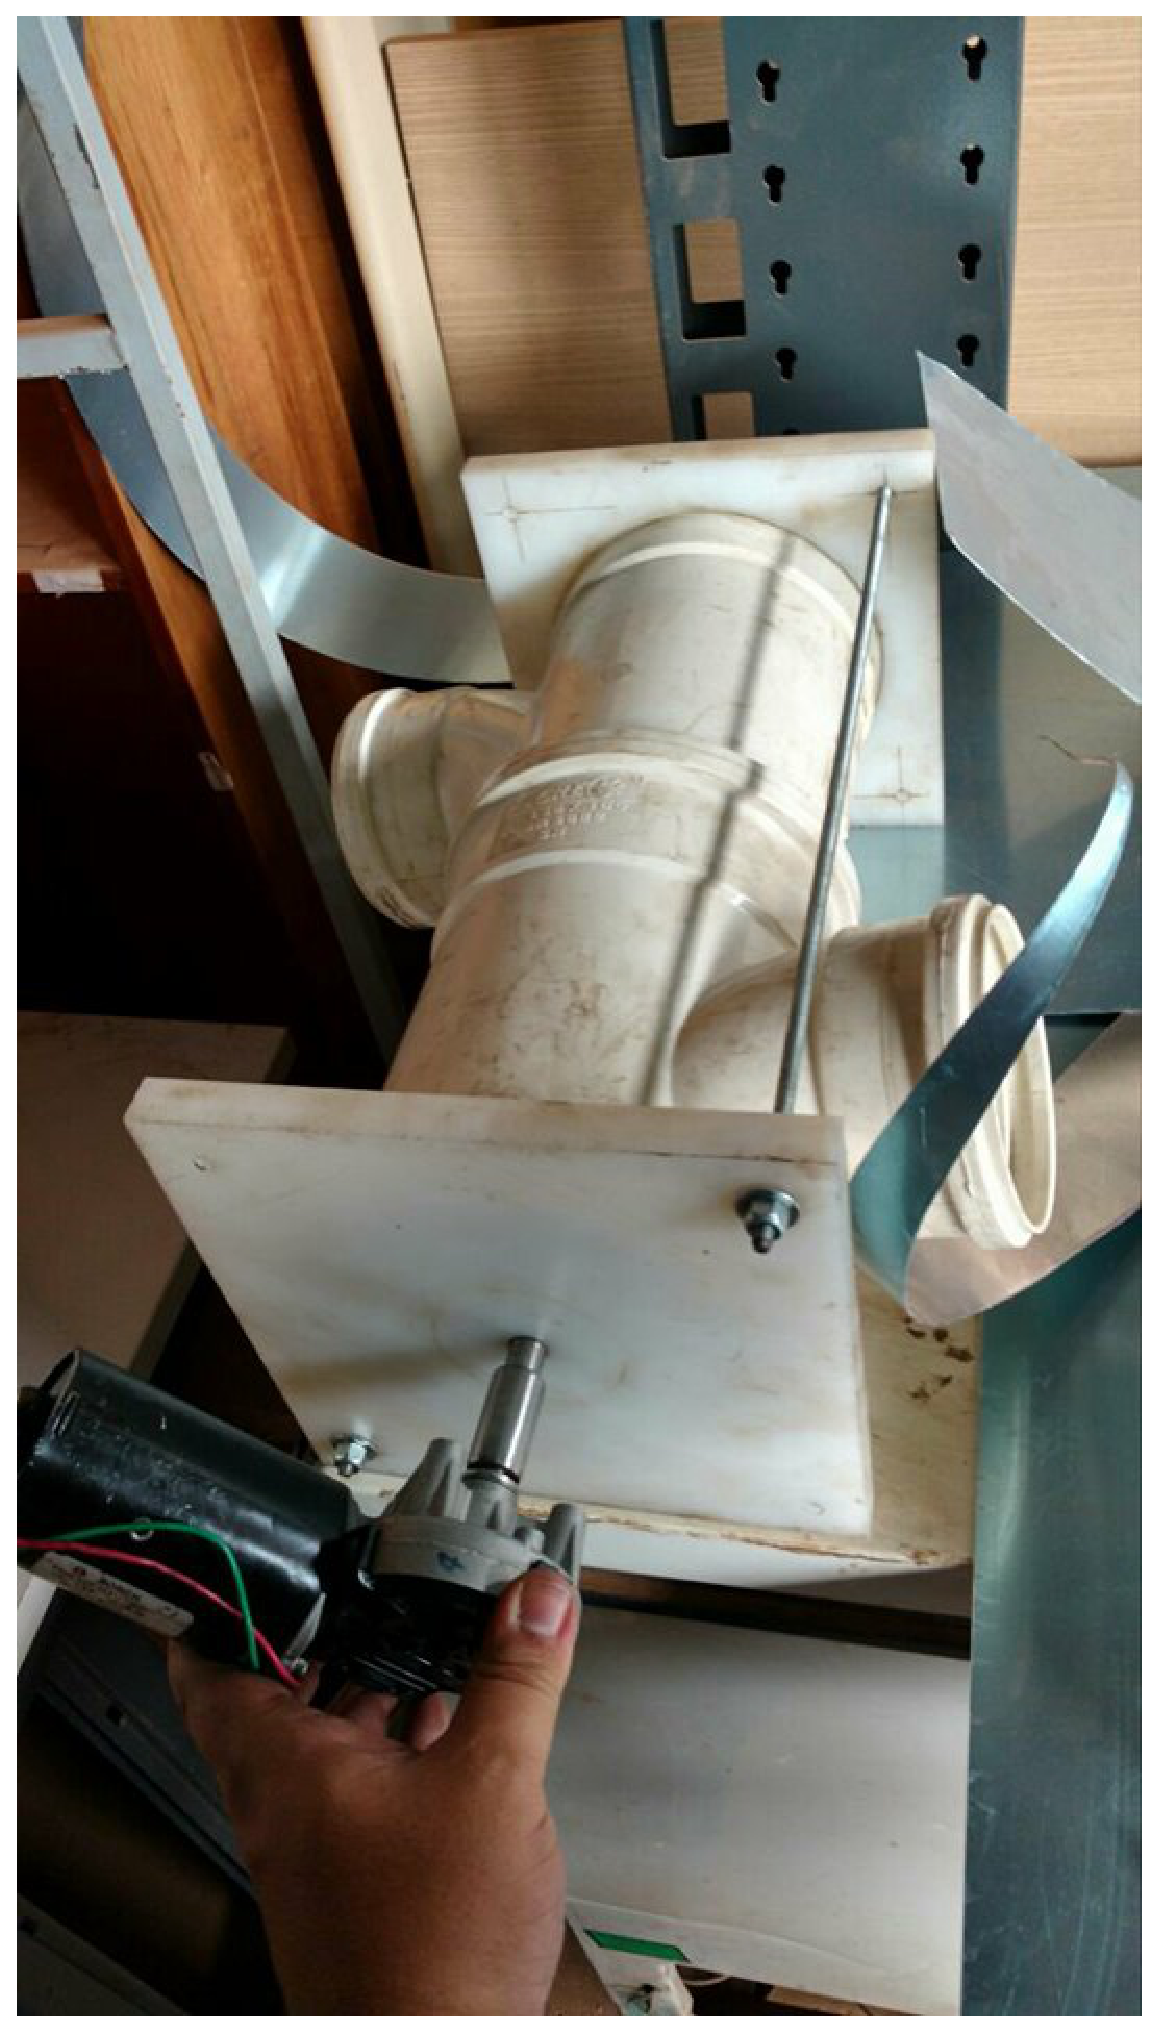
\includegraphics[scale=0.3]{figuras/motor}
\caption{Motor acoplado à rosca helicoidal}
\label{motor}
 \end{figure}

\subsection{Sistema de Alimentação de Energia}
O sistema de alimentação de energia será por meio de placa fotovoltaica, visto que o alimentador de peixes ficará no meio do lago, e não será possível fazer recarga de bateria. O sistema de geração é composto por:

\begin{itemize}
    \item Painel Solar Fotovoltaico
    \item Bateria
    \item Controlador de Carga
    \item Cabos para conexão do equipamento
    \item Suporte para o painel fotovoltaico

\end{itemize}

\subsubsection{Dimensionamento Sistema Fotovoltaico}
A grande vantagem da utilização da energia solar no projeto, é que esta é uma fonte renovável e sustentável. Além disso, o sistema tem um baixo custo de manutenção e longa vida útil. Quando houver energia excedente, a energia será armazenada na bateria estacionária. A seguir serão apresentados alguns dados necessários para o dimensionamento e o cálculo do número de módulos a ser utilizado no sistema.


\subsubsection*{Insolação}

A insolação da região de Dianópolis foi consultada no site da CRESESB, com valor médio de 4,94 Wh/$m^{2}$/dia.

\subsubsection*{Consumo diário do sistema}
O cálculo do consumo consiste na quantidade de watt-hora utilizada pelo motor e pelos componentes eletrônicos:
\\

$19~W*3h~=57~Wh/dia~\rightarrow~\text{Motor}$

$3~W*24h~=72~Wh/dia~\rightarrow~\text{Eletrônica}$
\\

Portanto, o valor total de consumo do sistema é de $57+72=129~Wh/dia$, ou 0,129 kWh/dia.

\subsubsection*{Características da Placa}
Informações como área, eficiência e potência da placa foram retiradas do próprio fabricante Yingli e podem ser observadas na tabela a seguir.

\begin{table}[!ht]
\centering
\caption{Características da Placa Fotovoltaica Yingli}
\label{my-label}
\begin{tabular}{|c|c|c|}
\hline
\textbf{Potência} & \textbf{Eficiência} & \textbf{Área} \\ \hline
20 W & 11,5\% & 0,1728 $m^{2}$ \\ \hline
\end{tabular}
\end{table}

\subsubsection*{Cálculo do número de módulos}
O número de módulos/placas que o sistema necessitará é calculado a partir da fórmula a seguir:


\begin{equation}
N_{\text{módulo}}= \frac{\text{Consumo por dia}}{\text{Insolação}\times~\text{Eficiência}~\times\text{Área da placa}}
\end{equation}

Onde:
\begin{equation}
N_{\text{módulo}}= \frac{0,129}{4,94\times0,115\times0,1728} = 1,31
\end{equation}

Observa-se que o ideal seria utilizar 2 módulos, porém como o trabalho foca no protótipo, será utilizado apenas uma placa, da marca Yingli.

FOTO DA PLACA

\subsubsection{Bateria}

Será necessária a utilização de uma bateria como de alimentação de motores e componentes eletrônicos do projeto, devido à incapacidade na utilização de energia elétrica e na praticidade ao utilizar a energia solar já disponível no local.

A bateria é utilizada nos sistemas fotovoltaicos para armazenar energia excedente produzida pelos painéis, para ser utilizada durante a noite ou em dias nublados ou com baixa insolação. As mais utilizadas em sistemas de energia renovável são as do tipo estacionárias ou de ciclo profundo, pois suportam grandes descargas que uma bateria comum não suportaria.


\begin{itemize}
\item{Dimensionamento da Bateria}
\end{itemize}

Conforme a potência total requerida pelo sistema (motor + componentes eletrônicos), 19 W + 2 W, calculou-se a corrente necessária.

Cálculo da corrente:

\begin{equation}
P_\text{motor}=19~W
\end{equation}

\begin{equation}
P_\text{eletrônica}=2~W
\end{equation}

\begin{equation}
P_{total}=P_\text{motor}+P_\text{eletrônica}=21~W
\end{equation}

\begin{equation}
i=\frac{P}{V}
\end{equation}

\begin{equation}
i\text{(motor)}=\frac{19}{12} = 1,58\,A
\end{equation}

\begin{equation}
i\text{(eletrônica)}=\frac{2}{12} = 0,166\,A
\end{equation}

Considerando a autonomia de 2h para o motor, e 24h para os componentes eletrônicos, calculou-se a capacidade da bateria.

\begin{equation}
\text{Capacidade}=(1,58\times2h).(0,166\times24h)=7,144~Ah
\end{equation}

Assim, a capacidade da bateria é 7,144 Ah, porém não é recomendado a descarga total, devido reduzir a vida útil da bateria. Considerando uma descarga de 75\%, calculou-se a capacidade para bateria.

Cálculo Capacidade da Bateria:

\begin{equation}
Ah=\frac{7,144\,Ah}{0,75}
\end{equation}

\begin{equation}
Ah=9,525
\end{equation}

Através do dimensionamento realizado a partir dos cálculos mostrados acima, foi escolhido uma bateria de 12Ah, como mostram as figuras abaixo:

\begin{figure}[!ht]
\centering
    \subfloat [a]{
        \includegraphics[keepaspectratio=true,scale=0.15]{bateria1}
        \label{Figura3} %esse é o nome da figura (a)
    }
    \qquad
    \subfloat[b]{
        \includegraphics[keepaspectratio=true,scale=0.15]{bateria2}
        \label{Figura4} %esse é o nome da figura (b)
    }\\

   \caption{Bateria}
\label{figuras1}
\end{figure}

\subsubsection{Controlador de Carga}
Será utilizado um controlador de carga acoplado aos painéis
fotovoltaicos e a bateria para realizar o controle do sistema.O controlador é responsável pela duração da vida útil dos bancos de baterias protegendo-o contra sobretensões e descargas excessivas. Assim, é de fundamental importância a utilização de um controlador de cargas. Esses controladores se localizam entre painéis fotovoltaicos e baterias onde controla-se a tensão de entrada já que as baterias não suportam grande flutuação de energia. Sendo assim, permite que as baterias sejam carregadas de melhor forma informando o estado de carga da bateria \cite{serrao2010dimensionamento}.
Para o dimensionamento do controlador, utiliza-se o consumo total do sistema (129 Wh) e a tensão da bateria (12V):

\begin{equation}
CC=\frac{129~Wh}{12~V}
\end{equation}

\begin{equation}
CC=10,75~A
\end{equation}

O cálculo acima mostra que para a quantidade de placas calculada para o sistema, seria necessário utilizar um controlador de carga acima de 10A, porém como será utilizado apenas uma placa no protótipo, e por questões de orçamento, foi escolhido o controlador de 10A, como mostram as figuras abaixo:

\begin{figure}[!htb]
\centering
    \subfloat [a]{
        \includegraphics[keepaspectratio=true,scale=0.15]{controlador1}
        \label{Figura3} %esse é o nome da figura (a)
    }
    \qquad
    \subfloat[b]{
        \includegraphics[keepaspectratio=true,scale=0.15]{controlador2}
        \label{Figura4} %esse é o nome da figura (b)
    }\\

   \caption{Controlador de carga}
\label{figuras1}
\end{figure}


    Características do controlador de carga solar SR 10A HP2410 – PWM:

    \begin{itemize}
\item{Identificação automática de sistemas de tensão 12/24V;}
\item{Visor LED digital com um sistema de interação simplificado, tornando seu manuseio simples e conveniente;}
\item{Estende a vida útil da bateria através da sua tecnologia de algoritmo de ponta.}
\item{Possuí quatro modos operacionais;}
\item{Alta durabilidade, podendo ser utilizado em ambientes hostis;}
\item{Saída 5V para USB, pode ser usada para carregar equipamentos eletrônicos como o celular;}
\item{Possui diversos tipos de indicações de status;}
\item{Periodicamente ou quando detectado descarregamento profundo da bateria, o controlador opera em modo equalizador, de forma a evitar sulfuração e desbalanceamento da bateria, o que aumenta efetivamente sua vida útil.}

\end{itemize}


\subsection{Dimensionamento dos Fios}
\par Os fios elétricos são especificados por um número, em função da carga elétrica por eles suportável. De acordo com a NBR 5410 da ABNT, podemos dimensionar a bitola do fio condutor da seguinte maneira:
\begin{equation}
s= \frac{L*P}{\sigma \times e\times {U}^{2}}
\end{equation}

\par Os fatores que influênciam no dimensionamento da bitola do fio a ser utilizado em um projeto são: a distância que a corrente elétrica tem de percorrer ao longo do fio (dada em metros), a potência do sistema (dada em Watts), a queda de tensão (considerada de 3\% para sistemas CC e 5\% para sistemas AC), a tensão de trabalho (V) e a condutividade elétrica dos cabos (condutividade elétrica do cobre é 56 metros por ohms milimetros ao quadrado.

\begin{equation}
s= \frac{2*129}{56 \times 0,03\times {12}^{2}}
\end{equation}
\par Logo a bitola do fio necessária para suportar o sistema é de:
\begin{equation}
s= 1,06 mm^2
\end{equation}
\par Então o condutor mais indicado para este projeto seria o condutor com bitola de no mínimo 1,5 mm, pois é o condutor com seção comercializada que vem logo acima do valor da capacidade calculada. Este condutor suporta uma corrente de até 15 amperes sem aquecer.
\par A capacidade de condução de energia de um condutor pode ser definida como  a maior corrente, em regime permanente, que ele suporta sem que a temperatura do mesmo ultrapasse a temperatura máxima suportada pela isolação.
\par O dimensionamento incorreto, resulta na diminuição da eficiência e no sobreaquecimento do fio que, em consequência, pode resultar em curto-circúito, perigo de choques e incêndio.


\subsection{Próximos Passos}
O motor acoplado à rosca helicoidal, bateria, placa fotovoltaica e controlador de carga já foram testados individualmente e em conjunto, ambos com sucesso. Os próximos passos do grupo de energia são relatados a seguir:

\begin{itemize}
    \item{Construção do suporte do sistema fotovoltaico;}
    \item{Integração com o subsistema de eletrônica;}
    \item{Integração com a estrutura.}
\end{itemize}
